\tolerance=10000
\hbadness=10000
\vbadness=10000

%\documentclass[aps,prl,twocolumn,showpacs,superscriptaddress,floatfix,10pt]{revtex4-1}
\documentclass[aps,prl,twocolumn,superscriptaddress,floatfix,10pt]{revtex4-1}
\usepackage{graphicx}% Include figure files
\usepackage{dcolumn}% Align table columns on decimal point
\usepackage{bm}% bold math
\usepackage{amsfonts}
\usepackage{amssymb}
\usepackage{amsmath}
%\usepackage{bbold}
\usepackage{fix-cm}
\usepackage{mathptmx} % rm & math
\usepackage[T1]{fontenc}
\usepackage[colorlinks,allcolors=blue]{hyperref}
%\usepackage{placeins}
%\raggedbottom
% no line skip between bibliography items like the production
\setlength{\bibsep}{0.0pt}
% remove the extra blank between multiple citations [a, b]===>[a,b] like in production
\makeatletter
\def\NAT@def@citea{\def\@citea{\NAT@separator}}
\makeatother

\begin{document}

\title{Dependence of fusion on isospin dynamics}

\author{K. Godbey}\email{kyle.s.godbey@vanderbilt.edu}
\affiliation{Department of Physics and Astronomy, Vanderbilt University, Nashville, TN 37235, USA}

\author{A.S. Umar}\email{umar@compsci.cas.vanderbilt.edu}
\affiliation{Department of Physics and Astronomy, Vanderbilt University, Nashville, TN 37235, USA}

\author{C. Simenel}\email{cedric.simenel@anu.edu.au}
\affiliation{Department of Nuclear Physics, Research School of Physics and Engineering, The Australian National University, Canberra ACT  2601, Australia}

\date{\today}

\begin{abstract}
We introduce a new microscopic approach to calculate the dependence of fusion barriers and cross-sections on
isospin dynamics. The method is based on the time-dependent Hartree-Fock theory and
the isoscalar and isovector properties of the energy density functional (EDF). The contribution to
the fusion barriers originating from the isoscalar and isovector parts of the EDF is calculated.
It is shown that for non-symmetric systems the isovector dynamics influence the sub-barrier fusion
cross-sections. For most systems this results in an enhancement of the sub-barrier cross-sections,
while for others we observe differing degrees of hindrance.
We use this approach to provide an explanation of recently measured fusion cross sections which show a  enhancement at low $E_\mathrm{c.m.}$ energies
for the system $^{40}$Ca+$^{132}$Sn as compared to the more neutron-rich system
$^{48}$Ca+$^{132}$Sn, and discuss the dependence of sub-barrier fusion cross-sections on transfer.

\end{abstract}
\pacs{25.70.Jj,24.10.Eq,21.60.Jz}
\maketitle

One of the major open questions in fusion reactions of exotic neutron-rich nuclei
is the dependence of the fusion cross section on the neutron excess,
or equivalently on the total isospin quantum number $T_z = (Z-N)/2$.
This is a timely subject given the expected
availability of increasingly exotic beams at rare isotope facilities\,\cite{balantekin2014}.
The influence of isospin dynamics on fusion is also one of the key questions pertaining to the
production of superheavy elements using neutron rich nuclei\,\cite{loveland2007}.
Besides being a fundamental nuclear structure and reaction question, the answer to this inquiry
is also vital to our understanding of the nuclear equation of state (EOS) and symmetry energy\,\cite{li2014}.
The EOS plays a key role in elucidating the structure of exotic nuclei\,\cite{chen2015},
the dynamics of heavy ion collisions\,\cite{danielewicz2002,tsang2009},
the composition of neutron stars\,\cite{haensel1990,chamel2008,horowitz2004,utama2016}, and the mechanism of core-collapse supernovae\,\cite{bonche1981,watanabe2009,shen2011}.
The influence of isospin flow during heavy-ion reaction is usually discussed in term of the
$(N/Z)$ asymmetry of the target and projectile or the $Q$-values for nucleon transfer.

The presence of positive $Q-$value transfer channels has been shown to enhance sub-barrier fusion in various systems~\cite{jiang2014a}.
However, what affects the magnitude of this enhancement is still actively debated~\cite{kohley2011,kohley2013,kolata2012,jiang2015,liang2016}.
In particular, recent experiments carried out
with radioactive $^{132}$Sn beams and with stable $^{124}$Sn beams on
$^{40,48}$Ca~\cite{kolata2012} and $^{58,64}$Ni~\cite{kohley2011} targets have shown that the enhancement is observed at much lower cross-sections in the heavier (Ni+Sn) systems~\cite{jiang2015} than in the lighter (Ca+Sn) ones.
Various possible effects have been invoked to explain these observations~\cite{liang2016},
such as a larger role of dissipation due to the increase of the charge product $Z_1Z_2$ of the collision partners~\cite{wolfs1987,evers2011,rafferty2016}.
%J'en suis la
It is also known that for systems with $Z_1Z_2\gtrsim1600$, the so-called quasifission, where the nuclei re-separate after a significant mass transfer, strongly hinders fusion~\cite{toke1985}.

The effect of neutron transfer on fusion is traditionally described  within the coupled-channels (CC) method~\cite{rowley1992,esbensen1998,hagino2012}
and models incorporating intermediate neutron
rearrangements\,\cite{zagrebaev2003,zagrebaev2007c,karpov2015}.
These approaches, however, model the transfer process on a schematic way
and they require nuclear data which are often unknown for exotic nuclei.
New approaches are then needed to describe realistically the effect of both proton and neutron transfers on fusion of stable and exotic nuclei.
In particular, dissipation induced by transfer should be properly accounted for.

Here, we take a first step toward this ambitious theoretical program by investigating the overall effect of isospin dynamics induced mostly by neutron and/or proton transfer in collisions of asymmetric systems~\cite{dasso1985,chomaz1993,baran1996,baran2001,simenel2001,baran2005,simenel2007,baran2009,oberacker2012,umar2008a}.
In particular, we address the impact of isospin dynamics on fusion barriers and cross-sections using
the microscopic
time-dependent Hartree-Fock (TDHF) theory\,\cite{negele1982,simenel2012}
together with the density-constrained TDHF (DC-TDHF) method for calculating fusion barriers\,\cite{umar2006b}.
This choice is motivated by the fact that the TDHF approach has been used to successfully describe multinucleon transfer~\cite{simenel2010,simenel2012b,sekizawa2013,scamps2013a,bourgin2016}, as well as strongly damped reactions such as deep-inelastic collisions~\cite{koonin1977,simenel2011} and quasi-fission~\cite{wakhle2014,umar2015a,umar2016}, without relying on an {\it a priori} knowledge of the structure of the reactants.
Therefore, these microscopic dynamical calculations incorporate the fundamental mechanisms which are relevant for a realistic description of the effect of transfer on fusion, including with exotic beams.
As a first application, various systems from Ca+Ca to Ca+Sn are considered.

In the TDHF approximation the many-body wavefunction is replaced by a single
Slater determinant and this form is preserved at all times, implying that two-body correlations
are neglected.
In this limit, the
variation of the time-dependent action with respect to the single-particle states, $\phi^{*}_{\lambda}$, yields the most probable time-dependent path
in the multi-dimensional space-time phase space
represented as a
set of coupled, nonlinear, self-consistent initial value equations
for the single-particle states
\begin{equation}
h(\{\phi_{\mu}\}) \ \phi_{\lambda} (r,t) = i \hbar \frac{\partial}{\partial t} \phi_{\lambda} (r,t)
\ \ \ \ (\lambda = 1,...,A)\,,
\label{eq:TDHF}
\end{equation}
where $h$ is the HF single-particle Hamiltonian.
These are the fully microscopic time-dependent Hartree-Fock equations.

Almost all TDHF calculations employ the Skyrme EDF, which allows the total energy of the system to be represented
as an integral of the energy density ${\cal H}(\mathbf{r})$\,\cite{engel1975}
\begin{equation}
\label{eq:energy}
E = \int d^3\mathbf{r} {\cal H}(\mathbf{r})\,,
\end{equation}
which includes the kinetic,
isoscalar, isovector, and Coulomb terms \,\cite{dobaczewski1995}:
\begin{equation}
\label{eq:edensity}
{\cal H}(\mathbf{r}) = \frac{\hbar^2}{2m}\tau_0
+ {\cal H}_0(\mathbf{r})
+ {\cal H}_1(\mathbf{r})
+ {\cal H}_C(\mathbf{r})\,.
\end{equation}
In particular,
\begin{widetext}
\begin{equation}
\label{eq:efunctional}
{\cal H}_\mathrm{I}(\mathbf{r})
= C_\mathrm{I}^{\rho}            \rho_\mathrm{I}^2
+  C_\mathrm{I}^{   s}            \mathbf{s}_\mathrm{I}^2
+  C_\mathrm{I}^{\Delta\rho}      \rho_\mathrm{I}\Delta\rho_\mathrm{I}
+  C_\mathrm{I}^{\Delta s}        \mathbf{s}_\mathrm{I}\cdot\Delta\mathbf{s}_\mathrm{I}
+  C_\mathrm{I}^{\tau}      \left(\rho_\mathrm{I}\tau_\mathrm{I}-\mathbf{j}_\mathrm{I}^2  \right)
+  C_\mathrm{I}^{   T}      \Big(\mathbf{s}_\mathrm{I}\cdot
\mathbf{T}_\mathrm{I} - \tensor{J}_\mathrm{I}^2\Big)
+ C_\mathrm{I}^{\nabla J}  \Big(\rho_\mathrm{I}\mathbf{\nabla}\cdot\mathbf{J}_\mathrm{I}
+ \mathbf{s}_\mathrm{I}\cdot
(\mathbf{\nabla}\times\mathbf{j}_\mathrm{I})\Big)\,,
\end{equation}
\end{widetext}
where we have used the gauge invariant form suitable for time-dependent calculations.
The isospin index $\mathrm{I}=0,1$ for isoscalar and isovector energy densities, respectively.
The most common choice of Skyrme EDF restricts the density dependence of the
coupling constants to the $C_\mathrm{I}^{\rho}$ and $C_\mathrm{I}^s$ terms only.
These density dependent coefficients contribute to the coupling of isoscalar and isovector fields
in the Hartree-Fock Hamiltonian.
The isoscalar (isovector) energy density, ${\cal H}_0(\mathbf{r})$ (${\cal H}_1(\mathbf{r})$), depends on the isoscalar (isovector) particle
density, $\rho_0 = \rho_n + \rho_p$ ($\rho_1 = \rho_n - \rho_p$), with analogous expressions for other densities and
currents.
Values of the coupling
coefficients as well as their relation to the alternative parametrizations of the Skyrme
EDF can be found in\,\cite{dobaczewski1995}.
\begin{figure}[!htb]
\includegraphics*[width=7.0cm]{V_40_48Ca.pdf}
\caption{(Color online) For the $^{40}$Ca+$^{48}$Ca system;
	Total and isoscalar DC-TDHF potentials. The shaded region
	corresponds to the reduction originating from the isovector contribution to the energy
	density. The insert shows the isoscalar and isovector contributions to the interaction barrier
	without the Coulomb potential.
    The TDHF collision energy was $E_\mathrm{c.m.}=55$\,MeV.}
\label{fig:CaCa}
\end{figure}

The above form of the EDF is more suitable for studying the isospin dependence
of nuclear properties and have been employed in nuclear structure studies\,\cite{dobaczewski1995}.
In the same spirit we can utilize this approach to study isospin dependent effects in nuclear
reactions microscopically.
In particular, the density-constrained time-dependent Hartree-Fock (DC-TDHF) method\,\cite{umar2006b} can be
employed to study isospin effects on fusion barriers and fusion cross-sections.
The DC-TDHF approach calculates the nucleus-nucleus potentials $V(R)$ directly
from  TDHF dynamics and has been used to calculate fusion cross-sections for a wide range of
reactions\,\cite{umar2014a,simenel2013a,umar2012a,umar2006a,oberacker2010,umar2009a,jiang2015a}.
The basic idea of this approach is the following:
At certain times $t$ or, equivalently, at certain internuclear distances
$R(t)$, a static energy minimization
is performed while constraining the proton and neutron densities to be equal to the instantaneous
TDHF densities.
We refer to the minimized energy as the ``density constrained energy''
$E_{\mathrm{DC}}(R)$.
The ion-ion interaction potential $V(R)$ is obtained by
subtracting the constant binding energies
$E_{\mathrm{A_{1}}}$ and $E_{\mathrm{A_{2}}}$ of the two individual nuclei
\begin{equation}
V(R)=E_{\mathrm{DC}}(R)-E_{\mathrm{A_{1}}}-E_{\mathrm{A_{2}}}\ .
\label{eq:vr}
\end{equation}
The calculated ion-ion interaction barriers contain all of the dynamical changes in the nuclear
density during the TDHF time-evolution in a self-consistent manner.
As a consequence of the dynamics the DC-TDHF potential is energy dependent\,\cite{umar2014a}.
Using the decomposition of the Skyrme EDF into isoscalar and isovector parts [Eq.\,(\ref{eq:efunctional})],
we can re-write this potential as
\begin{equation}
V(R) = \sum_{\mathrm{I}=0,1} v_\mathrm{I}(R) + V_C(R)\,,
\end{equation}
where $v_\mathrm{I}(R)$ denotes the potential computed by using the isoscalar and isovector parts of
the Skyrme EDF given in Eq.\,(\ref{eq:edensity}) in Eq.\,(\ref{eq:vr}).
The Coulomb potential is also calculated via Eq.\,(\ref{eq:vr}) using the Coulomb energy
density.
\begin{figure}[!htb]
\includegraphics*[width=7.0cm]{V_16O_208Pb_ecm75.pdf}
\caption{(Color online) For the $^{16}$O+$^{208}$Pb system;
	(a) Total and isoscalar DC-TDHF potentials at $E_\mathrm{c.m.}=75$\,MeV. The shaded
    region corresponds to the reduction originating from the isovector contribution to
    the energy density.
    (b) Same as in (a) except for $E_\mathrm{c.m.}=90$\,MeV.
       (c) Same as in (a) except for $E_\mathrm{c.m.}=120$\,MeV.}
\label{fig:OPb}
\end{figure}
\begin{figure}[!htb]
\includegraphics*[width=7.0cm]{V_CaTi_Pb_stack_2.pdf}
\caption{(Color online) Isoscalar and isovector breakdown of the potential barrier for two
    systems at the same $E_\mathrm{c.m.}/V_B=1.065$;
    (a) $^{48}$Ca+$^{208}$Pb. The shaded region corresponds to the increase originating
    from the isovector contribution to
    the energy density.
    (b) Same as in (a) except $^{50}$Ti+$^{208}$Pb.
    The shaded region corresponds to the decrease originating from the isovector contribution to
    the energy density.}
 \label{fig:CaTi_Pb}
\end{figure}

We have used the DC-TDHF approach to study fusion barriers for a number of systems.
Calculations were done in a three-dimensional
Cartesian geometry with no symmetry assumptions\,\cite{umar2006c} and using the
Skyrme SLy4 EDF\,\cite{chabanat1998a}.
The three-dimensional Poisson equation for the Coulomb potential
is solved by using Fast-Fourier Transform techniques
and the Slater approximation is used for the Coulomb exchange term.
The box size used for all the calculations
was chosen to be $60\times 30\times 30$~fm$^3$, with a mesh spacing of
$1.0$~fm in all directions. These values provide very accurate
results due to the employment of sophisticated discretization
techniques\,\cite{umar1991a}.
\begin{figure}[!htb]
\includegraphics*[width=7.0cm]{V_Ca_Sn_stack.pdf}
\caption{(Color online) For     (a) $^{40}$Ca+$^{132}$Sn,
	                            (b) $^{48}$Ca+$^{132}$Sn
	                            %(c) $^{54}$Ca+$^{132}$Sn
	                            systems;
	Total and isoscalar DC-TDHF potentials. In (a) the blue shaded region
       corresponds to the reduction originating from the isovector contribution.
       In (b) we see no isovector effect. (c) the isovector effect is reversed
       causing hindrance as shown by the red shaded region.
The inserts show the isoscalar and isovector contributions to the interaction barrier without the Coulomb potential.
The TDHF collision energy was $E_\mathrm{c.m.}=120$\,MeV.}
\label{fig:CaSn_1}
\end{figure}
%\onecolumngrid
\begin{figure}[!htb]
\centering
\includegraphics*[width=7.0cm]{current.pdf}
\caption{(Color online) Neutron and proton current vectors in $^{40,48}$Ca+$^{132}$Sn at $E_\mathrm{c.m.}=120$\,MeV and at
	a separation  $R=11.5$\,fm between the fragments.}
\label{fig:current}
\end{figure}
%\twocolumngrid

In Fig.\,\ref{fig:CaCa} we show the total and isoscalar fusion barriers (both including the Coulomb contribution)
for the $^{40}$Ca+$^{48}$Ca system at $E_\mathrm{c.m.}=55$~MeV.
 For the Ca+Ca systems the energy dependence is relatively
weak\,\cite{keser2012,umar2014a,washiyama2008}.
The reduction of the isoscalar barrier is due to the isovector contribution. It is evident that
the isovector dynamics results in the narrowing of the fusion barrier, thus resulting in an enhancement of the sub-barrier
fusion cross-sections. The insert in Fig.\,\ref{fig:CaCa} shows the isovector and isoscalar components without the Coulomb contribution.
We have also calculated fusion barriers for the $^{40}$Ca+$^{40}$Ca and $^{48}$Ca+$^{48}$Ca systems, where the isovector contribution is
zero as expected from symmetry.
Irrespective of its isovector/isoscalar nature, the DC-TDHF potential is a way to represent the potential felt by the system at a given time. The relation between time and distance between the fragments then allow to represent the potential in the traditional manner, i.e., as a function of the internuclear distance. The fact that the isovector reduction occurs essentially inside the barrier indicates that the proton and neutron flows become larger for stronger overlap occurring in the later stage of fusion.

As an example of a more asymmetric system we performed calculations for the $^{16}$O+$^{208}$Pb system
at $E_{\mathrm{c.m.}}=75$\,MeV. Results are shown in Fig.\,\ref{fig:OPb}(a). Here we see a
substantial enhancement of sub-barrier fusion due to the isovector dynamics.
For this system we have performed further
calculations at c.m. energies of 90\,MeV and 120\,MeV shown in Fig.\,\ref{fig:OPb}(b-c).
As the beam energy  increases, the
relative contribution from the isovector component to the total barrier decreases, while the overall barrier height increases with
increasing energy. At TDHF energies much higher than the barrier height the total barriers approaches the frozen density
barrier\,\cite{washiyama2008,umar2014a}
due to the inability of the system to rearrange at that time-scale at which time the isovector contribution vanishes as well.
Next, we have calculated isoscalar and isovector breakdown of the potential barrier for two
systems at the same $E_\mathrm{c.m.}/V_B=1.065$ as shown in Fig.\,\ref{fig:CaTi_Pb}(a,b) for;
$^{48}$Ca+$^{208}$Pb system where the shaded region corresponds to the increase in the barrier
originating
from the isovector contribution to the energy density, and for the
$^{50}$Ti+$^{208}$Pb system where
the shaded region corresponds to the decrease in the barrier originating from the isovector
contribution to
the energy density.
The above results demonstrate the influence of isovector dynamics on typical fusion barriers.

We next look at Ca$+$Sn reactions.
The experimental observation of a sub-barrier fusion enhancement in the system $^{40}$Ca+$^{132}$Sn
as compared to more neutron-rich system $^{48}$Ca+$^{132}$Sn was the subject of a previous DC-TDHF study\,\cite{oberacker2013},
where it was shown that the fusion barriers for the two systems have essentially the same height but the fusion barrier for
the $^{48}$Ca+$^{132}$Sn system was much wider than that for the $^{40}$Ca+$^{132}$Sn system.
We see in Fig.\,\ref{fig:CaSn_1}(a) a strong reduction of the isoscalar barrier due to the isovector contribution. This behavior is similar to that of the previous
two systems albeit the isovector reduction is somewhat larger as shown in the insert of
 Fig.\,\ref{fig:CaSn_1}(a).
We then performed the same calculation for the $^{48}$Ca+$^{132}$Sn system as shown in Fig.\,\ref{fig:CaSn_1}(b).
The startling result is the vanishing of the isovector contribution. With no isovector reduction the fusion barrier for this
system is much wider than that for the $^{40}$Ca+$^{132}$Sn system for which substantial reduction occurs.
The absence of the isovector component for the $^{48}$Ca+$^{132}$Sn system could be a reflection of the negative $Q-$values
for neutron pickup. This is the first direct observation of this phenomena in microscopic calculations.

This may also explain why for the $^{48}$Ca+$^{132}$Sn system simply considering the $2^+$ and
$3^-$ excitations of the target and projectile in coupled-channel calculations is able to
reproduce the sub-barrier fusion cross-sections, whereas doing the same for the $^{40}$Ca+$^{132}$Sn system grossly under-predicts the cross-sections.
In Ref.\,\cite{kolata2012}, this was attributed to transfer
%the presence of significant transfer,
which manifests itself in the isovector dynamics.
In Fig.\,\ref{fig:CaSn_1}(c) we have also calculated the potential barriers for the theoretical
$^{54}$Ca+$^{132}$Sn reaction. Here, we see that the influence of the isovector component
is reversed, as indicated by the shaded region. This reversal leads to the widening of
the potential barrier, further hindering sub-barrier fusion.

In all the studied systems, we observe an isovector reduction in the presence of  positive $Q-$values for transfer channels.
This can be understood from the $C_\mathrm{I}^{\rho}            \rho_\mathrm{I}^2$ term in Eq.~(\ref{eq:edensity})
which quantitatively dominates.
When an isospin equilibration occurs (driven by positive $Q-$values),
the $I=1$ contribution gets reduced as $(\rho_p-\rho_n)^2$ decreases
in each fragment and $C_1^\rho$ is positive.
This also explains why, in systems with only negative Q-values, the isovector contribution to the potential
vanishes.
In very few cases, such as for the theoretical $^{54}$Ca+$^{132}$Sn reaction,
we even found an increase of the
potential which is attributed to more complex density dependencies of $H_1$ in Eq.~(\ref{eq:edensity}).

In order to investigate the role of transfer in more detail we have plotted  in Fig.\,\ref{fig:current}
 the microscopic TDHF neutron and proton currents for $^{40,48}$Ca$+^{132}$Sn
 at  $E_\mathrm{c.m.}=120$\,MeV and  at the nuclear separation $R=11.5$\,fm,
which is slightly inside the barrier but still corresponds to an early stage of the reaction.
%for the same collision energy used to calculate the barriers shown in Fig.\,\ref{fig:CaSn_1}
In $^{40}$Ca+$^{132}$Sn, neutrons flow from Sn to Ca (Fig.~\ref{fig:current}a) and protons from Ca to Sn (Fig.~\ref{fig:current}c),
compatible with the fact that there are many positive $Q-$value channels for these transfers to occur.
For $^{48}$Ca$+^{132}$Sn, which has no positive $Q-$value transfer channel,
we observe a convergence of neutrons towards the neck (Fig.~\ref{fig:current}b),
which is what we would expect in the fusion process.
This is also what is observed for protons in (Fig.~\ref{fig:current}d),
although there is a larger displacement of protons from Ca towards the
neutron-rich neck. %Nevertheless, this does not correspond to a transfer
%of protons as the proton flow in the tin is also directed towards the neck,
%which is compatible with the fact that there is no positive $Q-$value for
%proton transfer in this system.
%Examination of these currents shows that for
%the $^{40}$Ca+$^{132}$Sn system neutrons flow from $^{132}$Sn to
%$^{40}$Ca, whereas the proton flow is from $^{40}$Ca to $^{132}$Sn.
%Proton flow for the $^{48}$Ca+$^{132}$Sn system is similar, namely from $^{48}$Ca to
%$^{132}$Sn. However, we observe an interesting difference for the neutron flow in the
%$^{48}$Ca+$^{132}$Sn system, namely a bi-directional flow between the two systems.
%The dynamics of this bi-directional flow results in
As a result, the isovector current density in the neck region is an order of magnitude lower
for the $^{48}$Ca+$^{132}$Sn system in comparison to the $^{40}$Ca+$^{132}$Sn.
\begin{figure}[!htb]
	\centering
	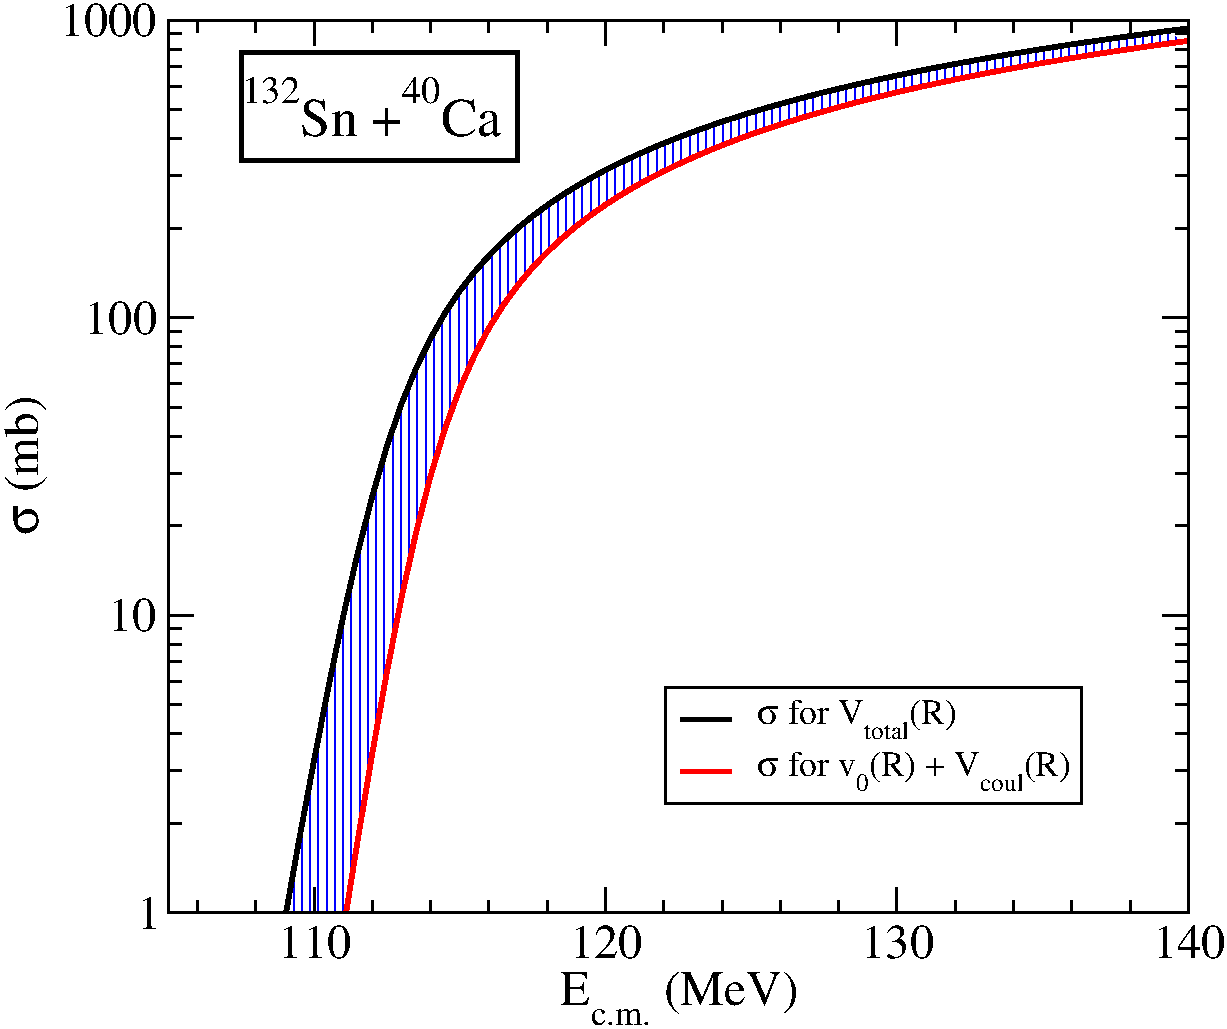
\includegraphics[width=7.0cm]{x_40Ca_132Sn.pdf}
	\caption{(Color online) Fusion cross-section  in $^{40}$Ca+$^{132}$Sn calculated with (black line) and without (red line) isovector reduction, using the potentials of Fig.~\ref{fig:CaSn_1}a.}
	\label{fig:cs}
\end{figure}
This is the primary cause for the disappearance of the isovector contribution to the barrier.
%In the neck region, the relative magnitude of the proton current density of $^{48}$Ca+$^{132}$Sn system
%is 30\%-50\% smaller than the proton current density of the $^{40}$Ca+$^{132}$Sn.
%This behavior is prevalent during the entire neck dynamics.
%Examination of the currents for the $^{54}$Ca+$^{132}$Sn reaction reveals that there is
%essentially no through-flow of neutrons or protons during the neck formation.

Finally, the impact of the isovector contribution to the fusion dynamics is shown in Fig.~\ref{fig:cs},
where fusion cross-sections have been computed from the DC-TDHF potentials of Fig.~\ref{fig:CaSn_1}a.
The effect of the isovector reduction is particularly visible at sub-barrier energies where an enhancement
of the fusion cross-sections by about an order of magnitude is observed.
To our knowledge, this is the first microscopic evidence of the enhancement
of fusion due to coupling to transfer channels.

In summary, we have developed a microscopic approach to study the effect of isospin dynamics on fusion barriers.
We have shown that for most systems isovector dynamics results in the thinning of the barrier thus enhancing
the sub-barrier fusion cross-sections. The isovector reduction effect vanishes for symmetric systems as well
as the $^{48}$Ca+$^{132}$Sn system for which neutron pickup $Q-$values are all negative.
These results provide a quantitative measure for the importance of transfer for
sub-barrier fusion reactions.
Furthermore, they elucidate the non-trivial dependence of sub-barrier fusion for neutron-rich
systems and illustrate the importance of dynamical microscopic models that incorporate the nuclear
structure and reactions on the same footing.
%A more detailed study including cross-section ratios and other systems will be the subject of a future study.

We thank K. Vo-Phuoc for useful discussions regarding the Ca+Sn systems.
This work has been supported by the U.S. Department of Energy under grant No.
DE-SC0013847 with Vanderbilt University and by the
Australian Research Council Grant No. FT120100760. 
%\FloatBarrier
\bibliography{VU_bibtex_master}

\end{document}
